\let\negmedspace\undefined
\let\negthickspace\undefined
\documentclass[journal,12pt,twocolumn]{IEEEtran}

\usepackage{csquotes}
\usepackage{comment}
\usepackage{enumerate}
\usepackage{amsmath,amssymb,amsthm}
\usepackage{graphicx}

\begin{document}
\graphicspath{{figures/}}

\title{Assignment 2 \\ \Large AI1110: Probability and Random Variables \\ \large Indian Institute of Technology Hyderabad}
\author{Busireddy Asli Nitej Reddy\\ \normalsize CS21BTECH11011  \\ \Large ICSE 2019 Grade 12}
\date{}
\maketitle


\begin{flushleft}

\section*{\textbf{Problem 2(A)}}
The following results were obtained with respect to two variable $x$ and $y$
       \newline
       $\sum x = 15$ , $\sum y = 25$ , $\sum xy = 83$
       \newline
       $\sum x^{2} = 55$ , $\sum y^{2} = 135$ , $\sum n = 5$
       
      \begin{enumerate}
         \item Find the regression coefficient $b_{xy}$
         \item Find the regression equation of $x$ on $y$
      \end{enumerate}



\section*{\textbf{Solution}}
   we are already given the 
       \newline
          $\sum x = 15$ , $\sum y = 25$ , $\sum xy = 83$
      \newline
          $\sum x^{2} = 55$ , $\sum y^{2} = 135$ , $\sum n = 5$
      \newline
   so let's start the part wise solutions
  
  
  
\subsection*{\textbf{Part 1}}
   in this part we need to find the regression coefficient $b_{xy}$
   \newline
   the formulae for calculating $b_{xy}$ is
   
      \begin{equation}
          \label{eq:b_xy}
          b_{xy}=\frac{\sum xy-\frac{{\sum x}\times  {\sum y}}{n} }{\sum y^{2}-\frac{(\sum y)^{2}}{n} }
      \end{equation}
      
   on substituting the values in eq\eqref{eq:b_xy} and simplyfying  we get 
 
      \begin{align}
          b_{xy}=\frac{83-\frac{15\times25}{5}}{135-\frac{(25)^{2}}{5} } = \frac{4}{5} = 0.8
      \end{align}
     
$\therefore$ the value of $b_{xy}$ is 0.8
 
 
 
 
\subsection*{\textbf{Part 2}}
 in this part we need to find the regression equation of $x$ on $y$
 \newline
 formulae for that is 
 
       \begin{equation}
           \label{eq:eq_x_on_y}
           x-\overline{x} = b_{xy}(y-\overline{y})
       \end{equation}
       
  where $\overline{x},\overline{y}$ are average of $x$ and $y$
 
       \begin{align}
           \overline{x} = \frac{\sum x}{n} = \frac{15}{5} = 3 \\
           \overline{y} = \frac{\sum y}{n} = \frac{25}{5} = 5
       \end{align}
    
  substituting values in eq\eqref{eq:eq_x_on_y} we get 
 
      \begin{align}
          x-3 = \frac{4}{5}(y-5) \\
          5x - 15 = 4y - 20 
      \end{align}
      
   final simplyfied equation is 
      \begin{equation}
          \label{eq:3}
          5x - 4y + 5 = 0
    \end{equation}
    
    
    
$\therefore$ regression equation of $x$ on $y$ is $5x-4y+5$ and the plot of eq\eqref{eq:3} is down below



\begin{figure}[h!]
		\centering
     	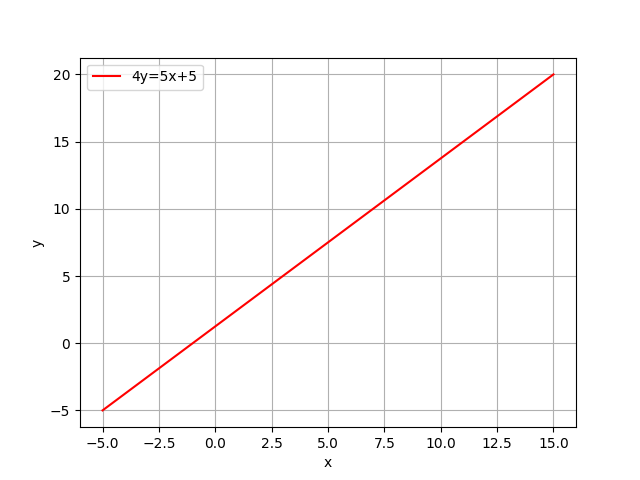
\includegraphics[width=\columnwidth]{figures/Figure_1.png}
    	\caption{graph of regression equation of $x$ on $y$}
	    \label{Fig1}
\end{figure}

\end{flushleft}

\end{document}
